\subsubsection{Thick shell gravity benchmark}
\label{sec:benchmark-thick-shell-gravity}

\textit{This section was contributed by Cedric Thieulot.}

This benchmark tests the accuracy of the gravity field and gravitational potential computed by the gravity postprocessor inside and outside an Earth-sized planet (without its core) of constant density. The domain is a spherical shell with inner radius $R\textsubscript{inner}=3840~\si{\km}$ and outer radius $R\textsubscript{outer}=6371~\si{\km}$. The density is constant in the domain and set to $\rho_0=3300~\si{\kg\per\cubic\metre}$.

First, let us calculate the exact profile which we expect the benchmark to reproduce. The gravitational potential $U$ of a spherically symmetric object satisfies the Poisson equation $\Delta U = 4\pi G \rho(\mathbf r)$. For a constant density shell, this equation can be solved analytically for the gravitational acceleration and potential inside and outside the planet.
Inside ($r<R\textsubscript{inner}$) and outside ($r>R\textsubscript{outer}$) the spherical shell (i.e. where $\rho=0$) the Poisson equation simplifies to the Laplace equation $\Delta U=0$:
\begin{equation}
\frac{1}{r^2} \frac{\partial }{\partial r} \left(r^2 \frac{\partial U}{\partial r} \right) = 0. 
\end{equation}
The solution to this expression is:
\begin{equation}
g=\frac{\partial U}{\partial r} = \frac{C}{r^2} \label{eq:app1},
\end{equation}
where $C$ is a constant of integration.
In order to avoid an infinite gravity field at $r=0$ (where the density is also zero in this particular setup of a shell), we need to impose $C=0$, i.e. the gravity is zero for $r\leq R\textsubscript{inner}$. Another way of arriving at the same conclusion is to realize that $g$ is zero at the center of the body because the material around it exerts an equal force in every direction.
Inside the shell, $\rho=\rho_0$, yielding
\begin{equation}
g=\frac{\partial U}{\partial r} = \frac{4 \pi}{3} G \rho_0 r + \frac{A}{r^2},
\end{equation}
where $A$ is another integration constant. 
At the inner boundary, $r=R\textsubscript{inner}$ and $g=0$, allowing $A$ to be computed. Substituting in the value of $A$,
\begin{equation}
g=\frac{\partial U}{\partial r} = \frac{4 \pi}{3} G \rho_0 
\left(r - \frac{R\textsubscript{inner}^3}{r^2} \right). \label{eqgin}
\end{equation}
When $r\geq R\textsubscript{outer}$, the gravitational potential is given by Eq. (\ref{eq:app1}). Requiring the gravity field to be continuous at $r=R\textsubscript{outer}$:
\begin{equation}
g(r) = \frac{G M}{r^2} \label{eq:gout},
\end{equation}
where $M=\frac{4 \pi}{3} \rho_0(R\textsubscript{outer}^3-R\textsubscript{inner}^3)$ is the mass contained in the shell.
For $r\ge R\textsubscript{outer}$, the potential is obtained by integrating Eq.(\ref{eq:gout}):
\begin{equation}
U(r)=-\frac{GM}{r} +D,
\end{equation}
where $D$ is an integration constant which has to be zero since we require the potential to vanish for $r\rightarrow \infty$.
The potential within the shell, $R\textsubscript{inner}\leq r \leq R\textsubscript{outer}$, is found by integrating Eq.~\eqref{eqgin}:
\begin{equation}
U(r)= \frac{4 \pi}{3} G \rho_0 \left(\frac{r^2}{2} + \frac{R\textsubscript{inner}^3}{r} \right)  + E,
\end{equation}
where $E$ is a constant. Continuity of the potential at $r=R\textsubscript{outer}$ requires that $E=-2\pi\rho_0 G R\textsubscript{outer}^2$. 
Gravitational acceleration is zero for $r\leq R\textsubscript{inner}$, so the potential there is constant and a continuity requirement yields
\begin{equation}
U(r)=2\pi G \rho_0 (R\textsubscript{inner}^2-R\textsubscript{outer}^2).
\end{equation}

The gravity postprocessor in \aspect{} can be used to calculate the radial components of gravity ($g_r$ and $U$) at arbitrary points using the sampling scheme `\textit{list of points}'. For this benchmark we calculate points along a line from the center of the planet to a distant point, $r=0$ to $r=10,000~\si{\km}$ (Figure \ref{fig:grav-thick-shell}). Arbitrarily, the latitude and longitude are both set to $13\si{\degree}$ so as to avoid potential measurement artifacts due to symmetry. The list of radii is defined as follows:

\lstinputlisting[language=prmfile]{cookbooks/benchmarks/gravity_thick_shell/doc/thick_shell.prm.out}

The resulting measurements obtained for a mesh composed of 12 caps of $32^3$ cells (i.e., 393,216 total mesh cells) are shown in Fig.~(\ref{fig:grav-thick-shell}) and are in good agreement with the analytical profiles.

\begin{figure}
  \centering
  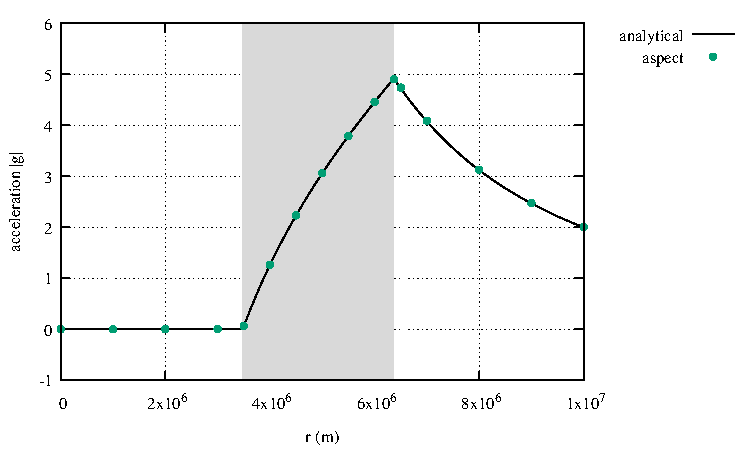
\includegraphics[width=8cm]{cookbooks/benchmarks/gravity_thick_shell/doc/gravity_g.pdf}
  \hfill
  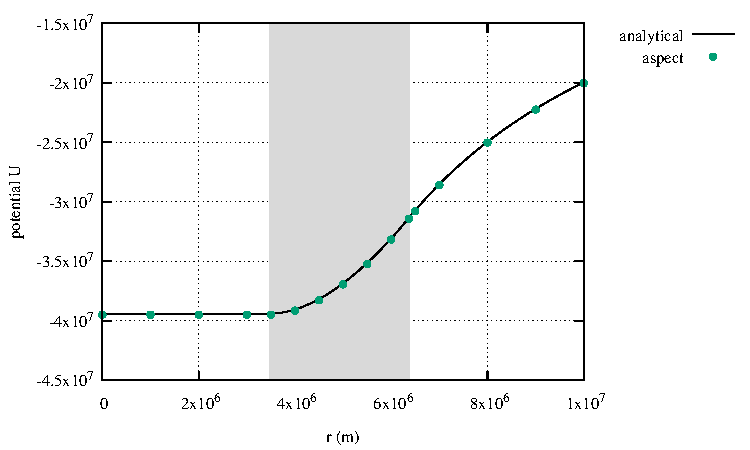
\includegraphics[width=8cm]{cookbooks/benchmarks/gravity_thick_shell/doc/gravity_U.pdf}
  \caption{\it Gravity benchmark for a thick shell: Gravitational potential (left) and acceleration (right) computed on a line from the center of a constant density shell to a radius of 10,000~\si{\km}. The gray area indicates the region $R\textsubscript{inner}\leq r \leq R\textsubscript{outer}$ inside the shell, where the density is not zero.}
  \label{fig:grav-thick-shell}
\end{figure}
